\chapter*{Conclusioni e sviluppi futuri}\label{ch:conclusioni}
\addcontentsline{toc}{chapter}{Conclusioni e sviluppi futuri}
Lo studio effettuato in questo lavoro di tesi ha evidenziato come le reti di sensori \textit{low-cost} per il monitoraggio della qualità dell'aria, come \textbf{AirQino} (\ref{sec:airqino}), possano rappresentare una soluzione efficace per il rilevamento dell'inquinamento atmosferico ad alta risoluzione sia temporale che spaziale. Queste soluzioni possono integrarsi con le reti di monitoraggio regionali già esistenti, che garantiscono misurazioni più accurate ma con un elevato costo di strumentazione, fornendo un quadro più completo della qualità dell'aria in ambiente urbano.

I risultati ottenuti mostrano che anche con sensori a basso costo è possibile misurare inquinanti come \ce{PM_{2.5}} e \ce{PM10} con una buona accuratezza, ancora migliore se si ha a disposizione un segnale di riferimento ARPAT con cui calibrare i sensori, applicando tecniche di regressione robusta ai modelli di regressione statistici. Per sensori a gas (come per il rilevamento di \ce{NO2}), invece, questo è risultato più complicato, anche se la fase di calibrazione ha comunque riportato miglioramenti significativi in termini di accuratezza.

Uno sviluppo futuro potrebbe essere quello di perfezionare il processo di calibrazione delle centraline, ad esempio aggiungendo ulteriori variabili in input modello di regressione, come la \textbf{temperatura} e l'\textbf{umidità} relativa, e verificare se questo porti ad un aumento dell'accuratezza della predizione.
 Questa idea trova riscontro nella figura \ref{fig:corr}, che mostra la matrice di correlazione tra \ce{PM_{2.5}}, \ce{PM10}, temperatura e umidità misurate dalla centralina SMART16 nel periodo 18/08/2020 - 30/08/2021. Dai dati si nota infatti che la temperatura tende a correlare negativamente con i PM (all'aumentare della temperatura  le polveri sottili tendono a calare), mentre l'umidità presenta l'effetto contrario.
		
\begin{figure}[H]
\centering
\captionsetup{justification=centering}
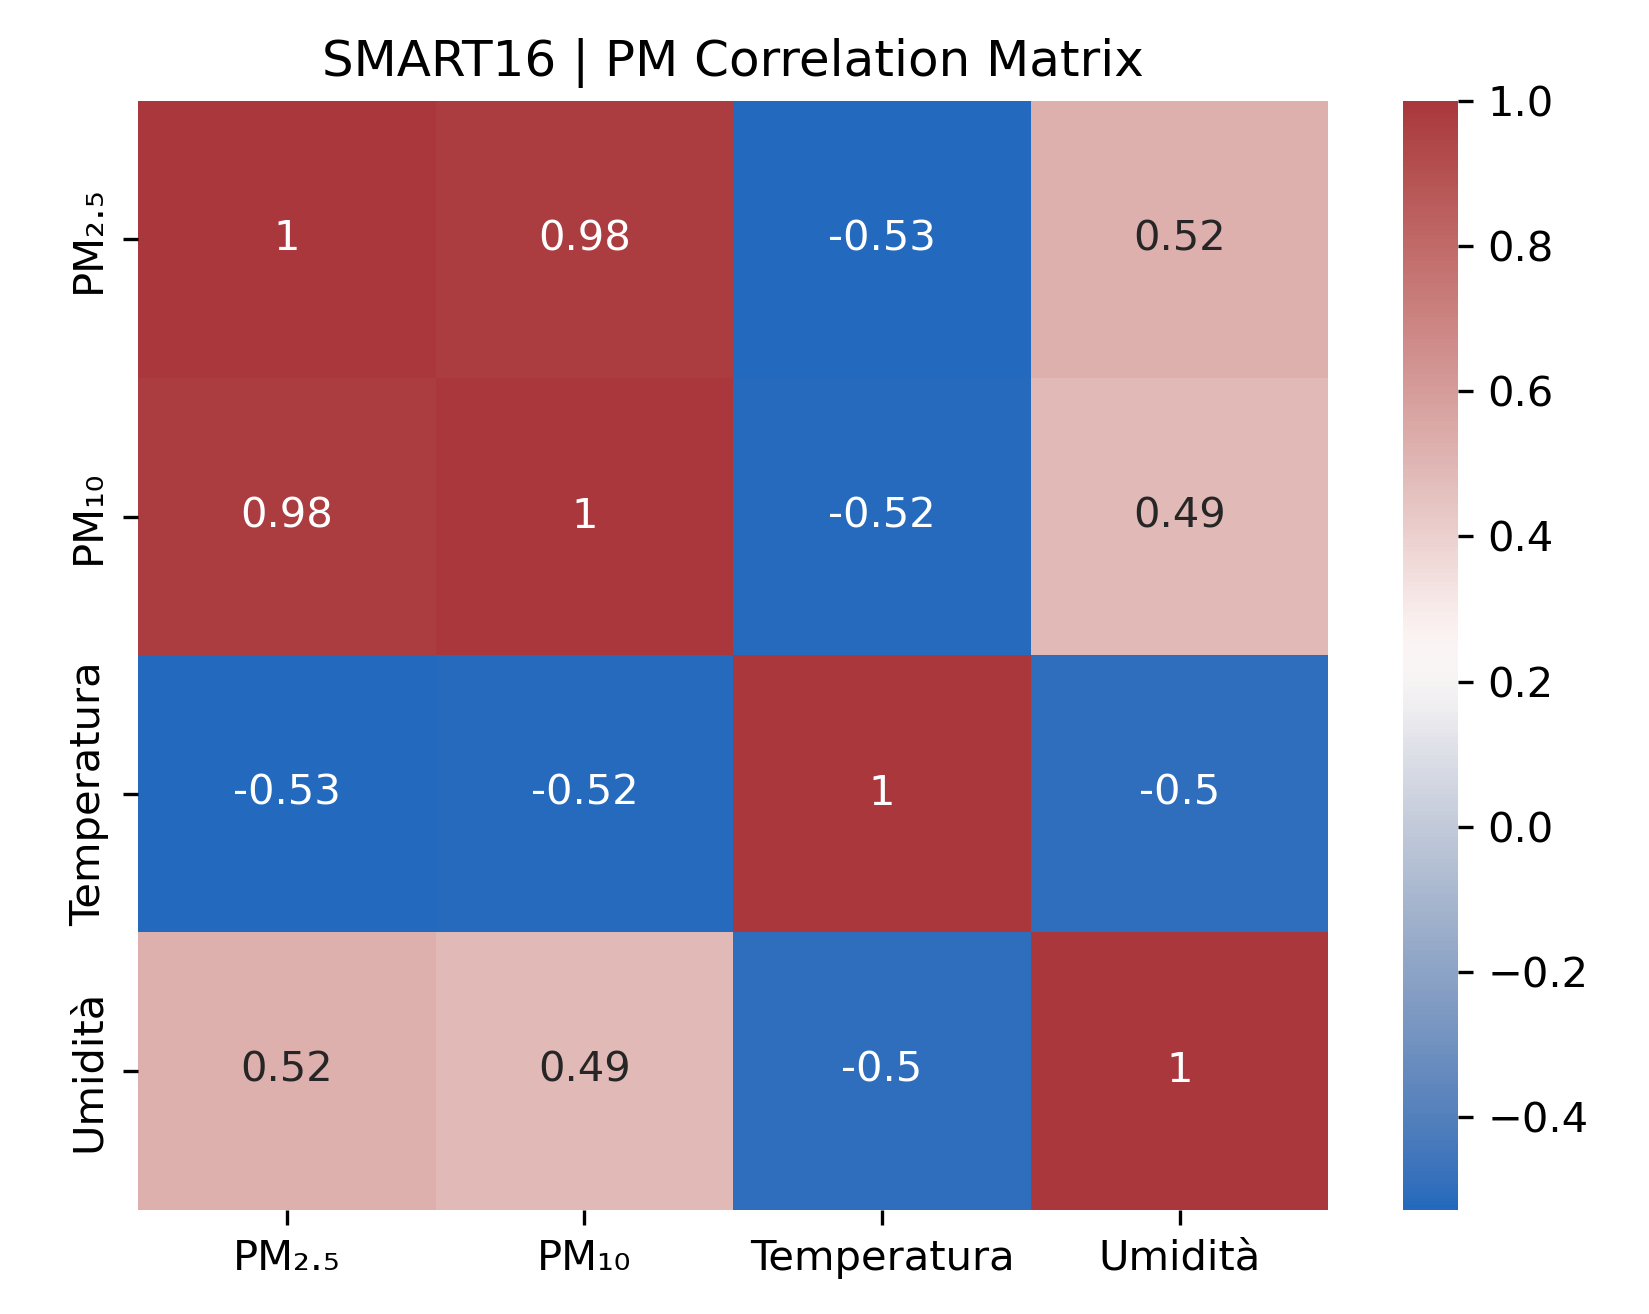
\includegraphics[width=0.70\textwidth,height=\textheight,keepaspectratio]{img/corr}
\caption{Correlazione tra polveri sottili, temperatura e umidità misurate dalla centralina SMART16 (AirQino) nel periodo 18/08/2020 - 30/08/2021}
\label{fig:corr}
\end{figure}

Come ulteriore sviluppo si potrebbe prevedere la realizzazione di una \textbf{procedura di allerta} sul segnale delle centraline. In particolare, effettuando un controllo in tempo reale sull'andamento del segnale e monitorando la differenza con il segnale di riferimento (es. stazione ARPAT), il sistema potrebbe inviare un messaggio di allerta nel caso in cui il segnale inizi a derivare, ovvero quando lo scarto tra i due non risulta più costante (ad esempio per l'usura del sensore), segnalando la necessità di una ricalibrazione.